\documentclass[
12pt,
a4paper,
twoside,
brazil
]{article}

\usepackage[brazil]{babel}
\usepackage[utf8]{inputenc}
\usepackage[T1]{fontenc}
\usepackage{lmodern}
\usepackage{hyperref}
\usepackage{amsmath}
\usepackage{indentfirst}
\usepackage[most]{tcolorbox}
\usepackage{inconsolata}
\usepackage{caption}
\usepackage{floatrow}
\usepackage[lined,algonl,ruled]{algorithm2e}
\usepackage{float}
\usepackage{graphicx,url}
\usepackage{subfigure}
\usepackage{times,epsfig}

\usepackage[
lmargin = 25mm,
rmargin = 25mm,
tmargin = 25mm,
bmargin = 25mm
]{geometry}

\author{Pedro Otávio Machado Ribeiro}
\title{Trabalho Prático 0\\Notação Polonesa Reversa\\Algoritmos e Estruturas de Dados III - 2017/01}
\date{20/04/2017}

\begin{document}
	
	\maketitle
	
	\section{Introdução}
	
	Neste trabalho, o problema proposto é descobrir todas as combinações possíveis de operações de soma e/ou multiplicação que satisfazem um dado resultado e imprimi-las em ordem lexicográfica na tela. Para isso, será fornecido expressões em \textit{RPN - Notação Polonesa Reversa} e um número correspondente ao resultado esperado.
	
	Foi necessário, primeiramente, compreender esta notação. Está possui o funcionamento simples, baseado nas operações da estrutura de dados pilha. Dada uma expressão, da esquerda pra direita, os operandos encontrados são inseridos na pilha, até que um operador seja identificado. Neste momento, os dois últimos operandos da pilha são retirados e a operação realizada. O novo resultado será também empilhado. E assim o processo se repete até que haja apenas um elemento na pilha, o qual será o resultado da expressão.
	
	Para solucionar o problema, o principal conceito necessário foi o de recursividade. A ideia da solução é inteiramente baseada nesta, para que as combinações de operadores possíveis sejam encontradas.
	
	\section{Metodologia}
	
	A solução proposta para o teste de combinações de operadores da expressão em \textit{RPN} utiliza duas estruturas de dados, sendo elas a pilha(\textit{stack}) e o vetor(\textit{vector}). Além disso, uma biblioteca com uma função para operar as operações em \textit{RPN} foi feita. A solução por si própria consiste apenas de uma função onde o algoritmo foi implementado.
	
	\subsection{Algoritmos}
	
	Os algoritmos implementados em linguagem C deste trabalho encontram-se dentro do diretório "src" presente neste mesmo diretório.
	
	\subsubsection{Operação em RPN}
	
	Realiza a operação em \textit{RPN}. Seu funcionamento é simples. Apenas retiro os dois últimos elementos da pilha para fazer o cálculo. Segue abaixo o pseudo-código:
	
	\hfill
	
	\begin{algorithm}[H]
		\begin{footnotesize}
			
			\eIf{operador soma} {
				soma os dois elementos do topo\;
			}{
				multiplica os dois elementos do topo\;
			}
			
			retorna resultado\;
			
			\caption{resolveRPN(pilha, operador)}
		\end{footnotesize}
	\end{algorithm}
	
	\subsubsection{Testa Combinações}
	
	Soluciona o problema em si. Dada a expressão com os operandos desconhecidos e o resultado esperado, o programa testa as combinações por meio da recursão. Para obter a solução de forma mais rápida, uma otimização no algoritmo foi feita de forma que a partir do momento que o resultado parcial for maior que o esperado, a chamada recursiva é retornada para que a próxima combinação seja testada. Dado que é feito a chamada recursiva primeiro para a soma e depois para a multiplicação, as combinações são testadas e impressas em ordem lexicográfica. Segue abaixo o pseudo-código do algoritmo:
	
	\begin{algorithm}[h!]
		\begin{footnotesize}
			
			\eIf{operador soma}{
				temp = resolveRPN(pilha, soma)\;
				\eIf{temp > resultado-esperado}{
					retorna\;
				}{
					insere(pilha, temp)\;
					concatena soma em combinação\;
				}
			}{
				temp = resolveRPN(pilha, multiplicação)\;
				\eIf{temp > resultado-esperado}{
					retorna\;
				}{
					insere(pilha, temp)\;
					concatena multiplicação em combinação\;
				}
			}
			
			\If{final da expr}{
				\If{topo-da-pilha = resultado-esperado} {
					imprime(combinação)\;
				}

				retorna\;
			}
			
			\While{houver operandos em expr}{
				insere(pilha, operando)\;
			}
			
			soluciona-problema(expr, soma, pilha, resultado, combinação)\;
			soluciona-problema(expr, multiplicação, pilha, resultado, combinação)\;
			
			\caption{soluciona-problema(expr, operador, pilha resultado-esperado, combinação)}
		\end{footnotesize}
	\end{algorithm}
	
	
	\section{Complexidade}
	
	Como trata-se de um problema onde devemos testar combinações, para cada operador desconhecido temos duas opções, soma ou multiplicação. Mesmo com a otimização que feita no código, o pior caso consiste em testar todas as possibilidades. Logo, a complexidade temporal da solução é $O(2^n)$, onde $n$ é a quantidade de operadores desconhecidos.
	
	Agora, em relação ao gasto de memória, seja $h$ a quantidade de operações desconhecidas e $n$ a quantidade de operandos na expressão em \textit{RPN}. Como o gasto de memória é linear, a complexidade espacial do algoritmo será $O(h*n)$.
	
	\section{Experimentos}
	
	Nesta seção, exibiremos os testes realizados, variando o tamanho e características das entradas. Os testes utilizados são de três naturezas: sequencia de 1s seguido de operações desconhecidas, com resultado variando de 1 a 9, ideia compartilhada pelo colega Pedro Gabriel, sequências alternadas de números aleatórios com resultado gerado aleatoriamente, ideia e gerador compartilhado pelo colega Igor Lucas, e, finalmente, situações específicas em sequências de 1s seguida de ?s onde o resultado é satisfeito por apenas uma combinação constituída de somas, que neste caso, é igual ao número de operandos.
	
	Os experimentos foram executados em um computador pessoal que possui sistema operacional Arch Linux, com processador Intel(R) Core(TM) i5-2430M 64 bits e 6GB de memória primária.
	
	Nos experimentos de expressões com sequências de 1s seguidos de ?s, foi utilizado o passo de 10 em 10, com 10 até 50 operações desconhecidas. Já no experimento  de expressões de operandos aleatorios alternados com operações desconhecidas, o passo foi de 5 em 5 partindo de 10 operações até 40 operações.
	
	Segue abaixo a tabela com os valores obtidos e em seguida o gráfico das duas situações:
	
	\begin{table}[H]
		\centering
		\caption{Tempos de Execução para a primeira situação}
		\label{table_sequencial}
		\begin{tabular}{|c|c|c|c|c|c|c|c|c|c|}
			\hline
			\#? / Resultado & \textbf{1} & \textbf{2} & \textbf{3} & \textbf{4} & \textbf{5} & 6    & 7     & 8      & 9      \\ \hline
			10              & 0.00       & 0.00       & 0.00       & 0.00       & 0.00       & 0.00 & 0.00  & 0.00   & 0.00   \\ \hline
			20              & 0.00       & 0.00       & 0.00       & 0.00       & 0.00       & 0.01 & 0.03  & 0.06   & 0.10   \\ \hline
			30              & 0.00       & 0.00       & 0.00       & 0.01       & 0.05       & 0.18 & 0.62  & 2.00   & 4.94   \\ \hline
			40              & 0.00       & 0.00       & 0.00       & 0.03       & 0.19       & 1.10 & 5.39  & 21.99  & 82.74  \\ \hline
			50              & 0.00       & 0.00       & 0.01       & 0.07       & 0.63       & 4.54 & 28.19 & 155.76 & 722.58 \\ \hline
		\end{tabular}
	\end{table}

	\begin{table}[H]
		\centering
		\caption{Tempo de Execução para segunda situação}
		\label{tabela_alternada}
		\begin{tabular}{|c|c|}
			\hline
			\textbf{\#?}                      & \textbf{Tempo de Execução (s)} \\ \hline
			\textbf{10}                       & 0.00                           \\ \hline
			\textbf{15}                       & 0.01                           \\ \hline
			\textbf{20}                       & 0.17                           \\ \hline
			\textbf{25}                       & 1.76                           \\ \hline
			\textbf{30}                       & 14.95                          \\ \hline
			\multicolumn{1}{|l|}{\textbf{35}} & 82.83                          \\ \hline
			\multicolumn{1}{|l|}{\textbf{40}} & 516.24                         \\ \hline
		\end{tabular}
	\end{table}
	
	\begin{figure}[H]
		\centering
		\subfigure[\label{tempo_sequencia_n_operacoes}]
		{
			\centering
			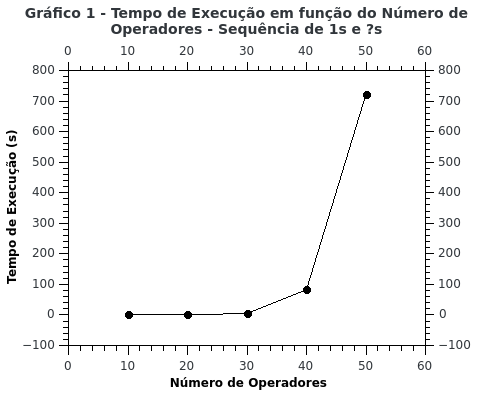
\includegraphics[width=3.0in,height=2.3in]{../graficos/grafico_1_sequencial.png}
		}
		\subfigure[\label{tempo_alternada_n_operacoes}]
		{
			\centering
			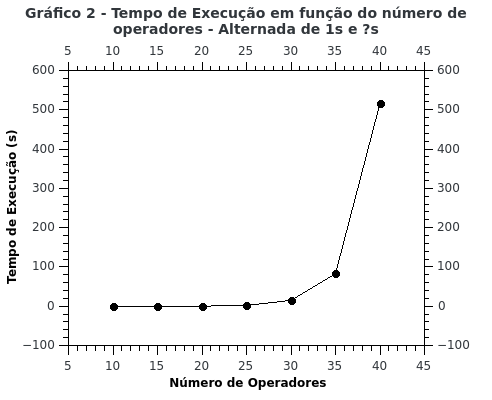
\includegraphics[width=3.0in,height=2.3in]{../graficos/grafico_2_alternada.png}
		}
		\caption{Tempo de execução para as duas situações propostas \label{tempo_n_operacoes}}
	\end{figure}

	A terceira situação mencionada consiste no pior caso do algoritmo. A otimização feita não é efetiva neste caso, e consequentemente, todos os casos são testados, pois a poda nunca ocorre. Devido a isso, em casos até mesmo pequenos, como por exemplo 30 operadores desconhecidos, o tempo se torna extremamente alto, e inviável de ser testado experimentalmente. Devido a isso, não foi possível coletar dados significativos para serem apresentados aqui neste documento.
	
	Os arquivos de imagem dos gráfico apresentados encontram-se no diretório "graficos". Os arquivos de casos de teste e logs de experimentos feitos encontram-se no diretório "testes".
	
	A contagem de tempo de execução foi automatizada por shellscripts utilizando a função time, do GNU Linux. Estes se encontram no diretório "scripts".
	
	Todos os diretórios mencionados estão no diretório raiz deste trabalho.
		
	\section{Análise de Resultado}
	
	Nota-se, para todas as situações de testes propostas, que há um crescimento exponencial no tempo de execução relacionado a quantidade de operadores desconhecidos cresce. Dessa forma, nota-se que o resultado condiz com a complexidade sugerida, que no caso é $O(2^n)$.
	
	Em relação a caractecterística das entradas, nota-se que no teste sequencial de 1s e ?s, há um grande número de combinções possíveis, que pode ser descrito pelo número combinatório $(h\ r)$, onde $h$ é o número de operações desconhecidas e $r$ é o resultado esperado.
	
	Os teste com operandos aleatórios alternados e resultado aleatório mostrou-se que possui um conjunto mais específico de combinações possíveis, de forma que é possível perceber que a distância lexicográfica é maior que no caso anterior.
	
	\section{Implementação}
	
	Todo o trabalho foi feito na linguagem C padrão. Cada arquivo contido no diretório "src" possui um cabeçalho explicando sua função.
	Para compilar, basta compilar o programa, basta utilizar o comando \textit{\$ make}.
	Para executar o programa, utilize o comando \textit{\$ ./tp0} .
	
	\section{Conclusão}
	
	Neste trabalho foi descrito uma solução para obter todas as combinações possíveis de operações, dada uma expressão em Notação Polonesa Reversa e um resultado esperado. A estratégia utilizada não foi muito sofisticada, devido à natureza do problema, em que é necessário buscar com força bruta a combinação que satisfaz o resultado. Uma melhoria feita na solução foi a poda de alguns galhos da árvore de recursão no momento em que o resultado experado é extrapolado, porém de nada adianta quando temos a situação mostrada na seção de experimentos.
	
	Este trabalho prático mostrou que a solução para o problema proposto é simples, porém não possui solução polinomial. Logo, qualquer solução proposta será pelo menos $\theta(2^n)$.
	
	O objetivo do trabalho prático foi alcançado. As combinações possíveis são encontradas e impressas na tela em posição lexicográfica.
	
	Alguns pontos podem ser melhorados nessa solução, como por exemplo a cópia de pilhas que faço para cada chamada recursiva. Sabe-se que é possível descrever uma solução onde isso não necessário, porém o autor deste trabalho não conseguiu fazê-lo desta forma.
	
\end{document}
